\section{Break‐Even Penetration Analysis}
\label{sec:Results_BreakEven}

The break-even study identifies the combinations of traffic volume and \ac{mpr} at which \ac{eco-glosa} yields lower mean \ac{co2} emissions than either the \ac{flow-glosa} baseline or the uncontrolled Standard scenario. The numerical results are listed in Tables~\vref{tab:BreakEven_EcoVsFlow} and \vref{tab:BreakEven_EcoVsStd}, while the decision maps are grouped in Figures~\vref{fig:BE_EcoFlow} and \vref{fig:BE_EcoStd}.

\paragraph{\ac{eco-glosa} versus \ac{flow-glosa}.}
A direct comparison between the two controllers reveals a complex relationship that is highly dependent on both traffic volume and the underlying emission model, as depicted in the table~\vref{tab:BreakEven_EcoVsFlow}. The performance of \ac{eco-glosa} under the HBEFA4 model is particularly volatile, as illustrated in Figure~\vref{fig:BE_EcoFlow_HBEFA4}. While it can offer a peak benefit of $+2.30~\unit{\gram\per\kilo\metre}$ at a very low demand of $69~\unit{\veh\per\hour}$, this advantage is not stable. At the same demand level but a higher penetration of $50\%$, it incurs a penalty of $-3.55~\unit{\gram\per\kilo\metre}$. This inconsistency persists at higher flows; for instance, at $692~\unit{\veh\per\hour}$, an initial benefit of $+11.68~\unit{\gram\per\kilo\metre}$ at $10\%$ \ac{mpr} eventually becomes a deficit of $-5.38~\unit{\gram\per\kilo\metre}$ at full penetration. In high-demand scenarios, the outcome is unequivocally negative, with penalties exceeding $-350~\unit{\gram\per\kilo\metre}$. This demonstrates that for the HBEFA4 model, the effective operational window for \ac{eco-glosa} is narrow and unpredictable.
\mynewline
The PHEMlight5 model provides a clearer performance separation, as seen in Figure~\vref{fig:BE_EcoFlow_PHEM} and table~\vref{tab:BreakEven_EcoVsStd}. In this case, the \ac{eco-glosa} strategy is consistently superior in low-demand and low-penetration scenarios. It achieves positive margins for nearly all \ac{mpr} values at demands up to $692~\unit{\veh\per\hour}$, with a peak benefit of $+8.46~\unit{\gram\per\kilo\metre}$ recorded at $346~\unit{\veh\per\hour}$. However, the controller becomes markedly and consistently inferior as soon as traffic density increases further. Beginning at a demand of $1385~\unit{\veh\per\hour}$, its performance enters a near-universal deficit. This penalty becomes severe in congestion, reaching as high as $-197.81~\unit{\gram\per\kilo\metre}$ at $3462~\unit{\veh\per\hour}$ and $60\%$ \ac{mpr}. The clear and steep penalty under the PHEMlight5 model stems directly from its superior transient engine map, which more accurately amplifies the high fuel cost of the sharp and frequent accelerations induced by \ac{eco-glosa} within queued traffic.

\begin{figure}[htb]
  \centering
  \begin{subfigure}[b]{0.45\textwidth}
    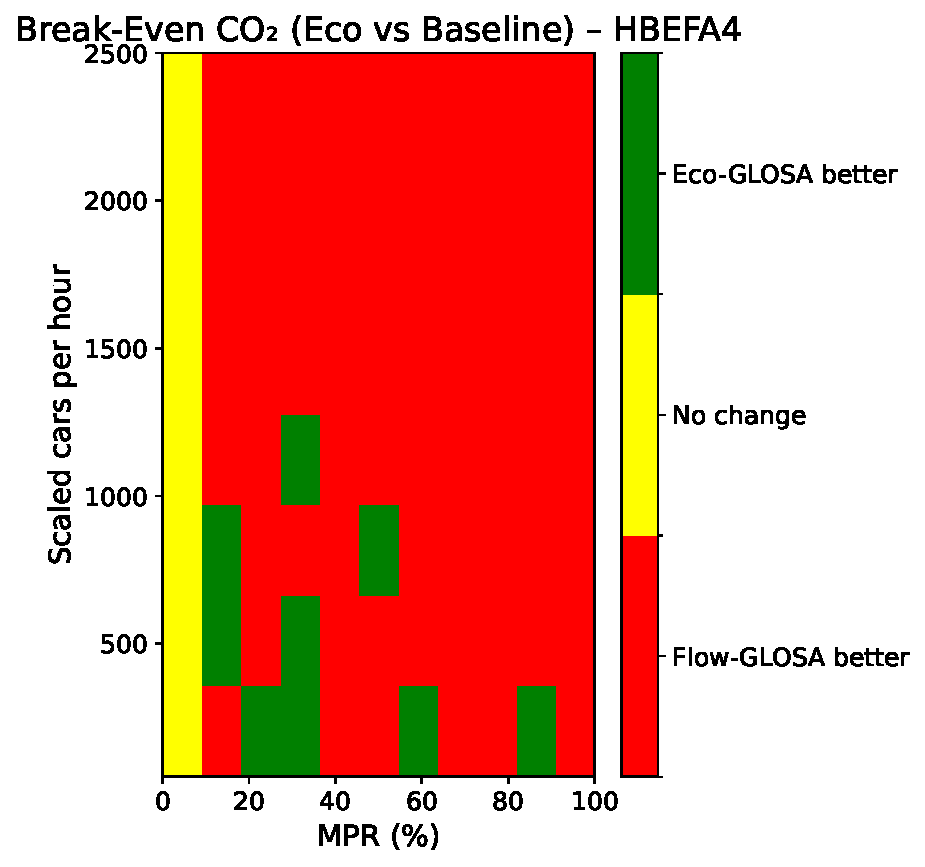
\includegraphics[width=\textwidth]{data/img/BreakEven/BreakEven_CO2_HBEFA4.pdf}
    \caption{Comparison using the HBEFA4 model.}
    \label{fig:BE_EcoFlow_HBEFA4}
  \end{subfigure}\hfill
  \begin{subfigure}[b]{0.45\textwidth}
    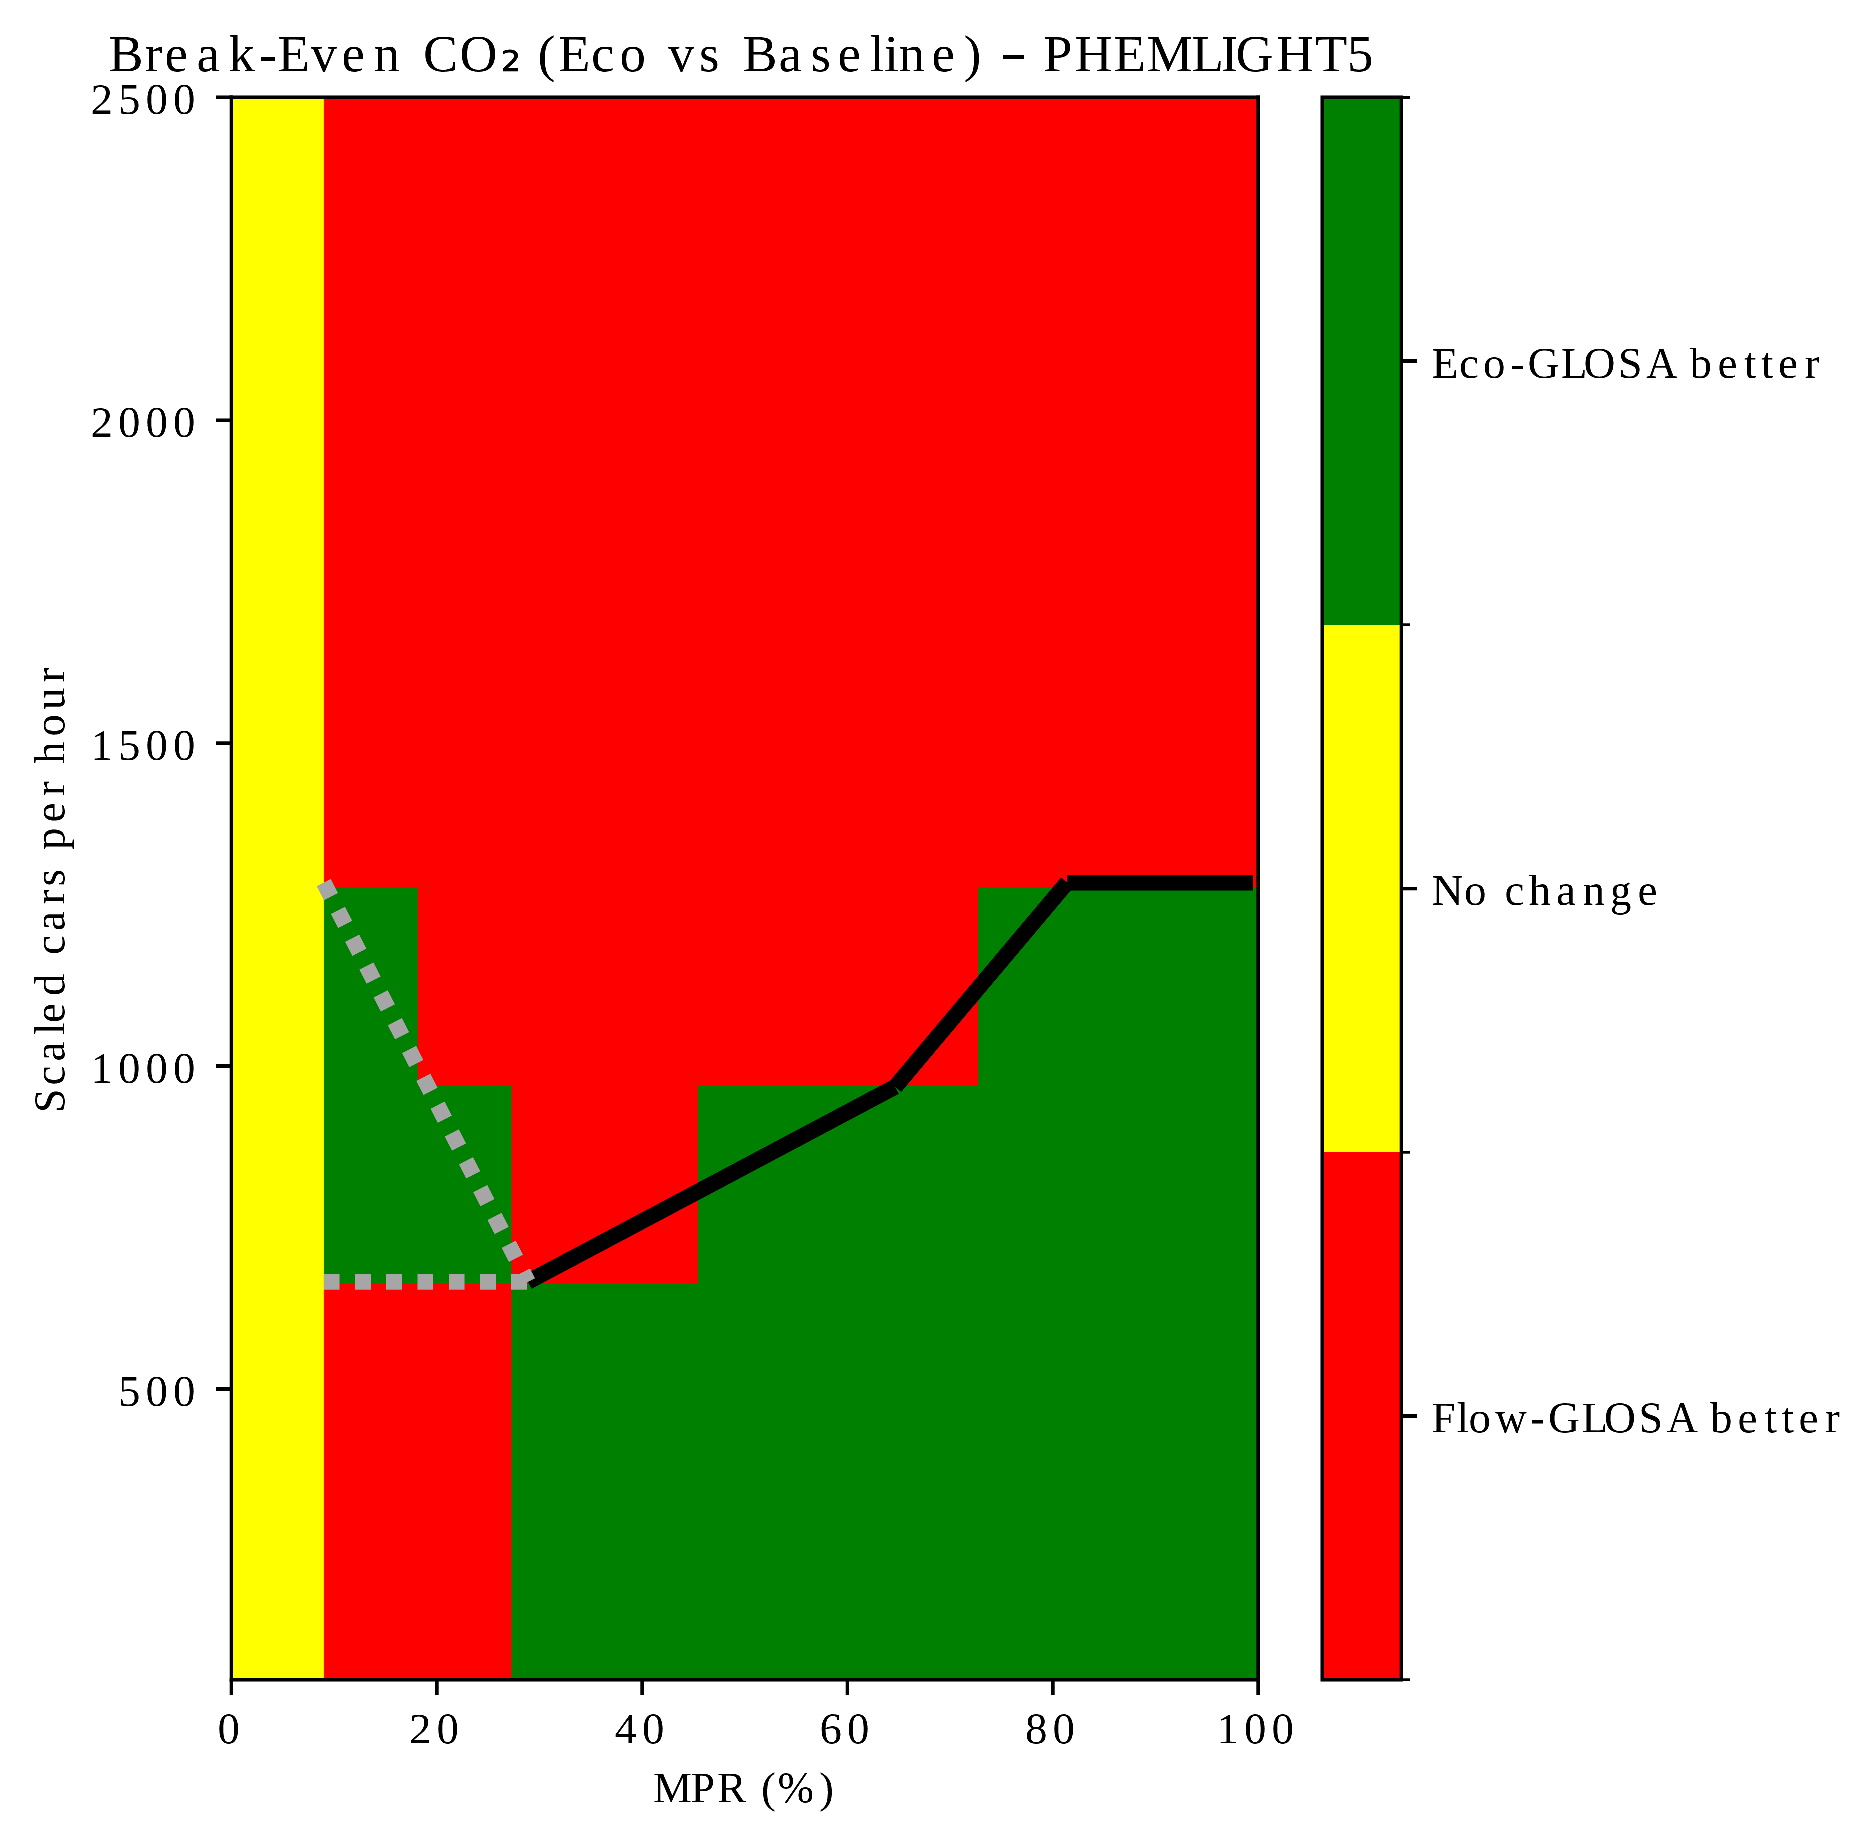
\includegraphics[width=\textwidth]{data/img/BreakEven/BreakEven_CO2_PHEMLIGHT5.pdf}
    \caption{Comparison using the PHEMlight5 model.}
    \label{fig:BE_EcoFlow_PHEM}
  \end{subfigure}
  \caption[Break-even CO2 map: Eco-GLOSA vs. Flow-GLOSA]{Break-even analysis of \ac{co2} emissions, comparing the performance of \ac{eco-glosa} against \ac{flow-glosa}. The heat map visualizes the performance difference across the full parameter space of traffic volume and \ac{mpr}. Green regions denote scenarios where \ac{eco-glosa} is superior (lower emissions), while red indicates that \ac{flow-glosa} is more fuel-efficient.}
  \label{fig:BE_EcoFlow}
\end{figure}

\paragraph{\ac{eco-glosa} versus Standard.}
When compared to the uncontrolled Standard scenario, \ac{eco-glosa} can deliver substantial emission reductions, though its effectiveness under the HBEFA4 model is highly conditional. As shown in Figure~\vref{fig:BE_EcoStd_HBEFA4}, it achieves sizeable gains in low and medium-volume traffic, with a peak reduction of $+22.11~\unit{\gram\per\kilo\metre}$ at $69~\unit{\veh\per\hour}$ and $40\%$ \ac{mpr}. However, the performance is volatile; even at this low demand, an \ac{mpr} of $20\%$ results in a net increase in emissions of $-19.38~\unit{\gram\per\kilo\metre}$. As demand increases towards saturation, this zone of benefit narrows considerably, becoming increasingly fragmented and eventually disappearing entirely.
\mynewline
Under the PHEMlight5 model, the performance of \ac{eco-glosa} is more consistent in lighter traffic, and the region of benefit is larger (Figure~\vref{fig:BE_EcoStd_PHEM}). It yields positive outcomes for most \ac{mpr} values for all demands up to $1385~\unit{\veh\per\hour}$. The maximum benefit reaches $+24.06~\unit{\gram\per\kilo\metre}$ at $69~\unit{\veh\per\hour}$ and $50\%$ \ac{mpr}, and even at $1385~\unit{\veh\per\hour}$, it still provides a respectable saving of $+11.17~\unit{\gram\per\kilo\metre}$. The transition is stark: for the two highest demand levels, the outcome becomes overwhelmingly negative as the controller fails to manage congestion. The worst-case performance is a severe penalty of $-163.38~\unit{\gram\per\kilo\metre}$ at $2769~\unit{\veh\per\hour}$ and $60\%$ \ac{mpr}, demonstrating that the potential benefits in light traffic are dwarfed by the severe consequences of applying this strategy in the wrong conditions.

\begin{figure}[htb]
  \centering
  \begin{subfigure}[b]{0.45\textwidth}
    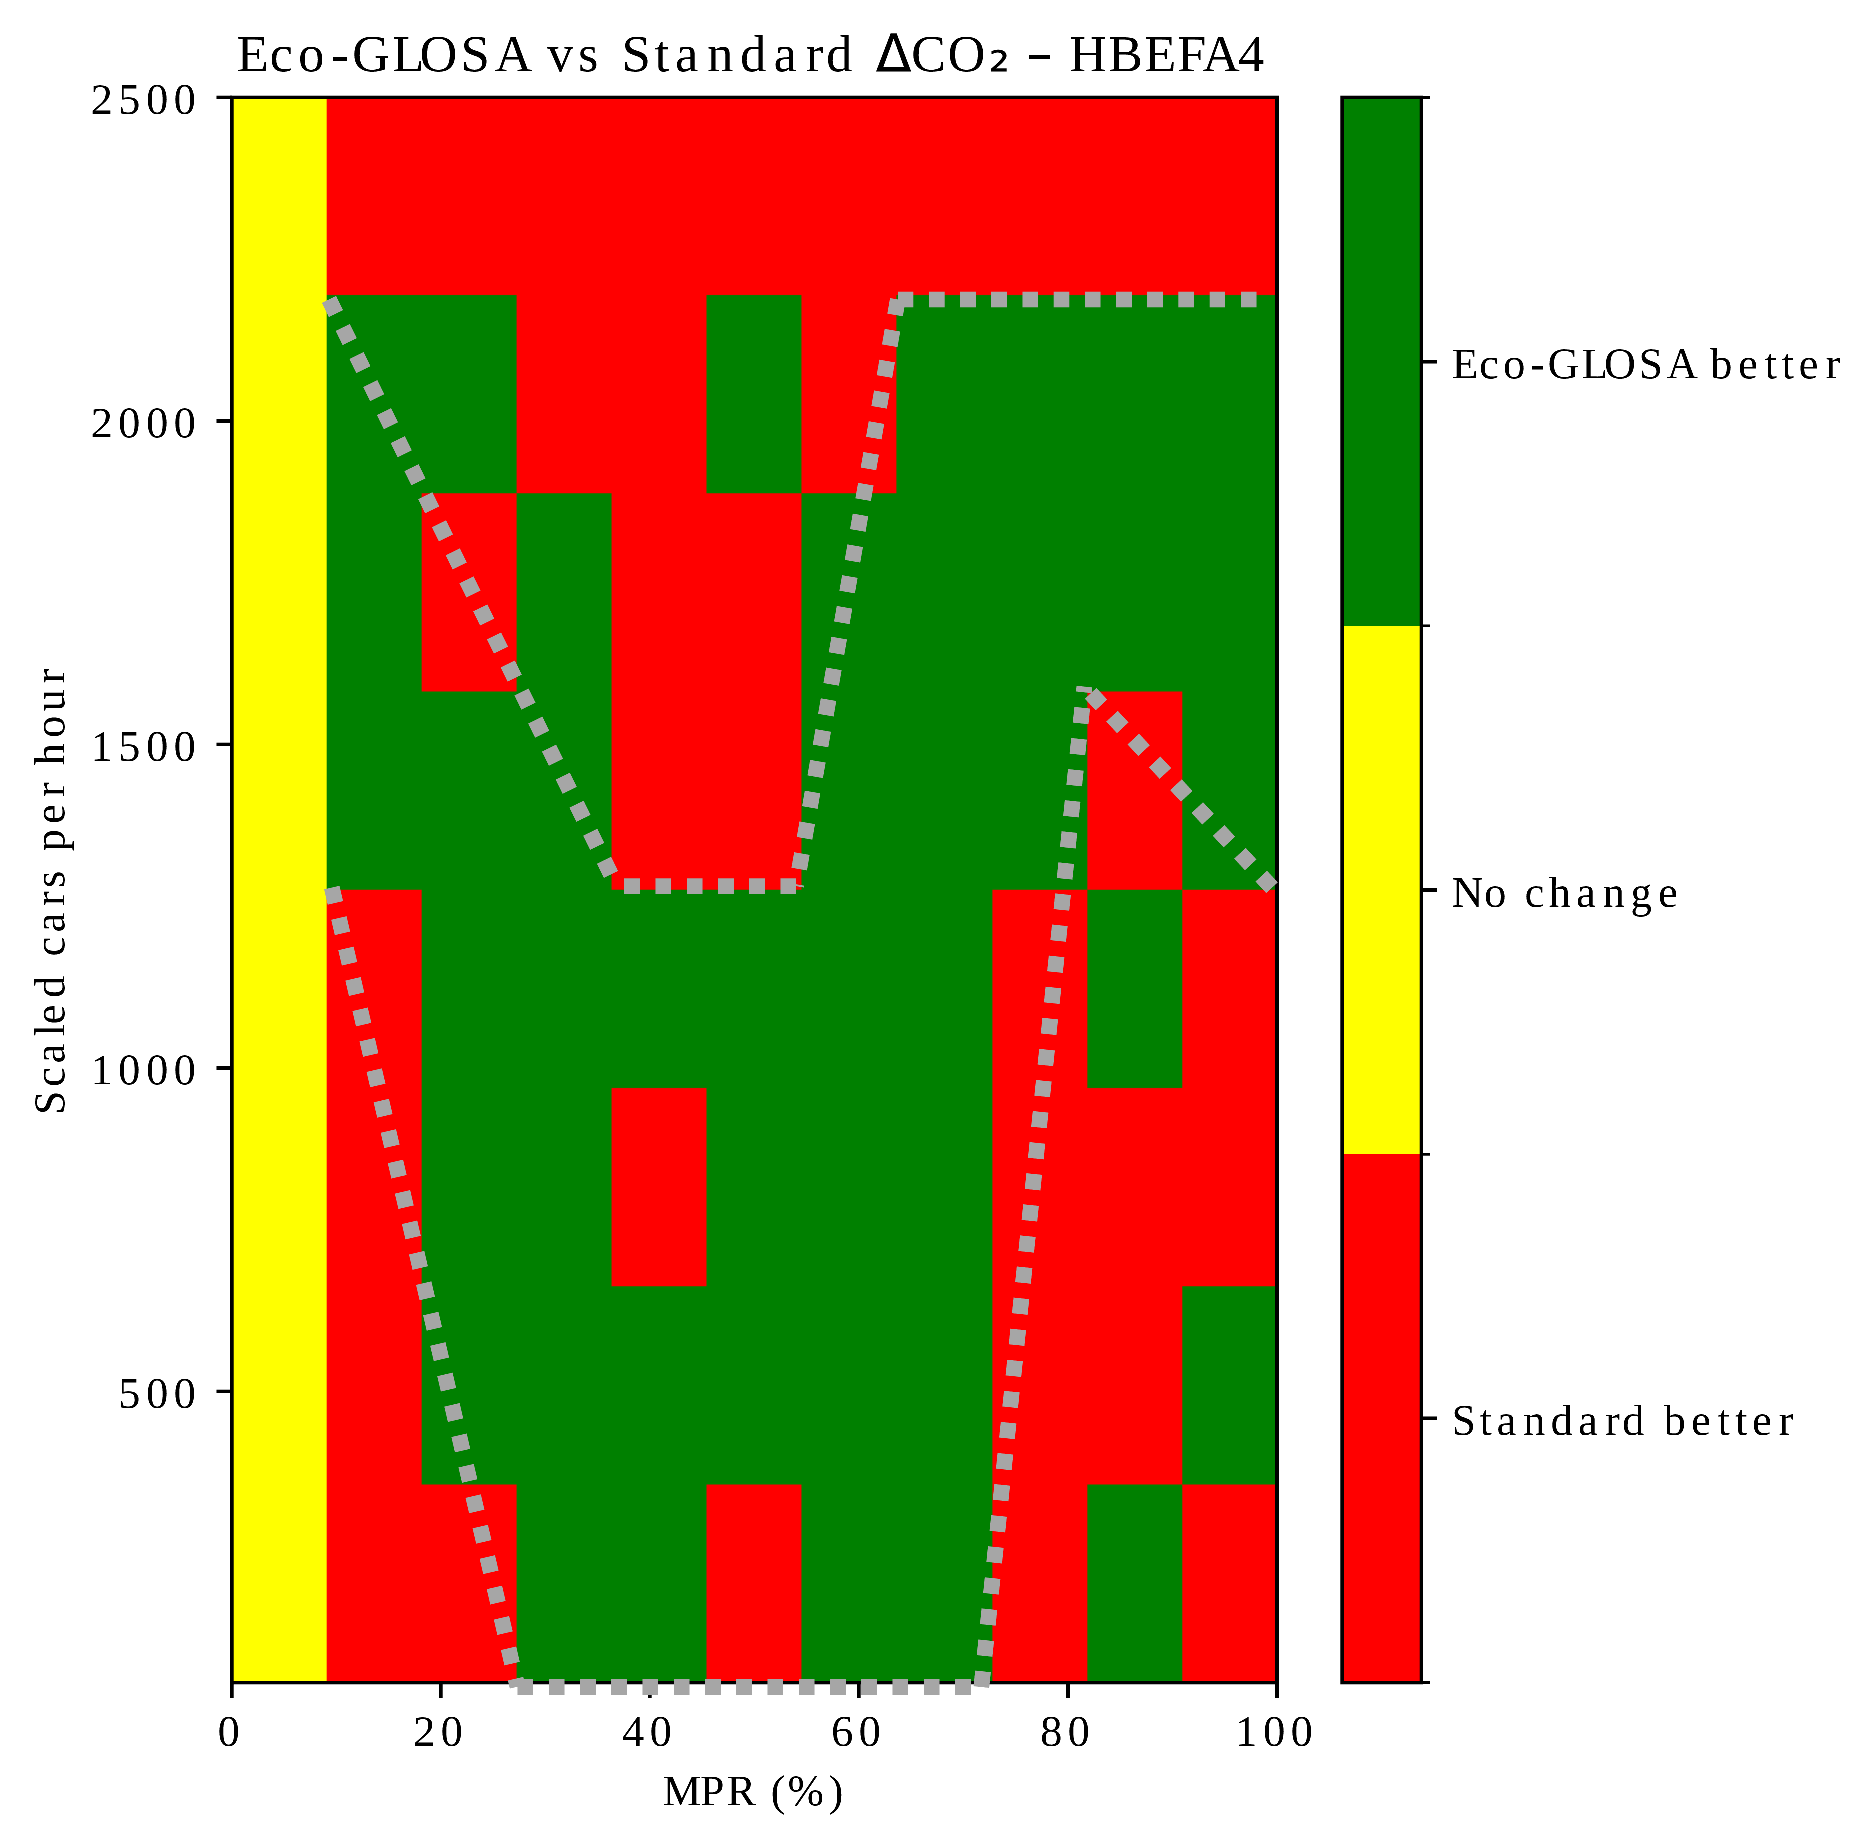
\includegraphics[width=\textwidth]{data/img/BreakEven/delta_CO2_HBEFA4.pdf}
    \caption{Results based on the HBEFA4 model.}
    \label{fig:BE_EcoStd_HBEFA4}
  \end{subfigure}\hfill
  \begin{subfigure}[b]{0.45\textwidth}
    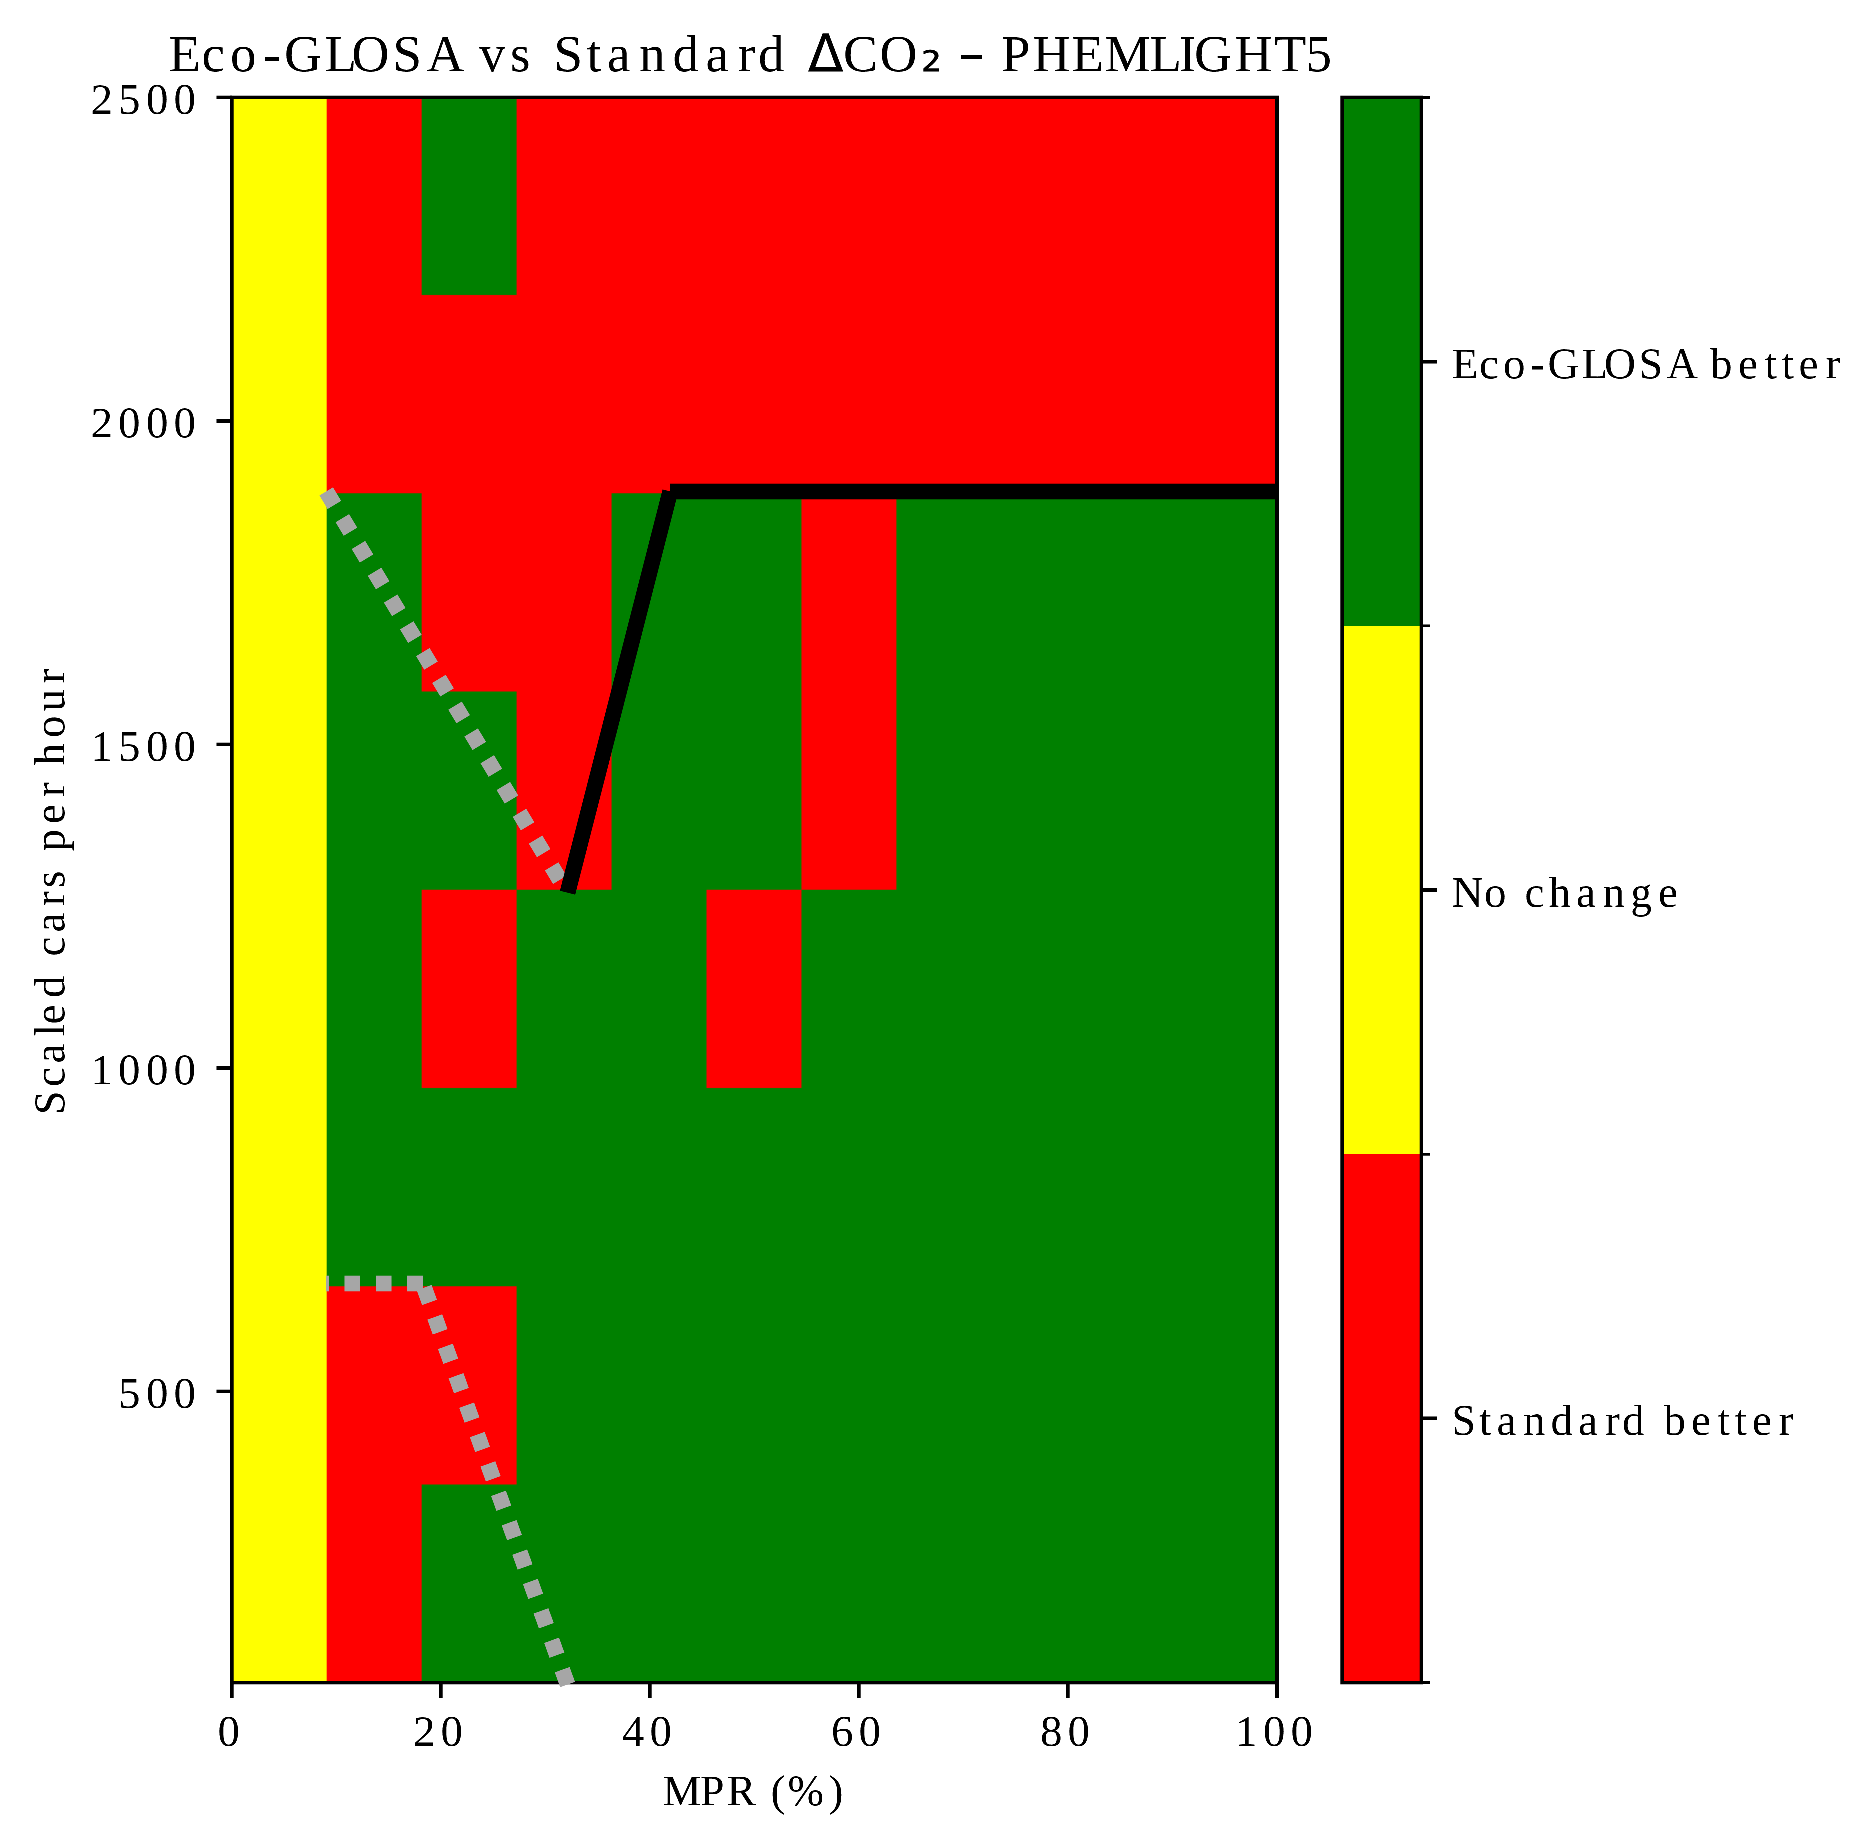
\includegraphics[width=\textwidth]{data/img/BreakEven/delta_CO2_PHEMLIGHT5.pdf}
    \caption{Results based on the PHEMlight5 model.}
    \label{fig:BE_EcoStd_PHEM}
  \end{subfigure}
  \caption[Relative CO2 performance of Eco-GLOSA vs. Standard]{Relative \ac{co2} emission performance of \ac{eco-glosa} compared to the Standard (uncontrolled) scenario. The heat map shows the outcome across all traffic volumes and \ac{mpr} values. Green regions represent a net reduction in emissions for \ac{eco-glosa}, whereas red regions indicate a net increase. The solid black curve traces the path of maximum emission reduction.}
  \label{fig:BE_EcoStd}
\end{figure}

\paragraph{Deployment Implications.}
These findings lead to a clear conclusion: the optimal controller strategy is regime-dependent, and the choice between controllers involves a critical trade-off between vehicle-level efficiency and network-level stability. The analysis delineates three distinct operational envelopes.
\mynewline
First, in lightly loaded corridors with demand below approximately $700~\unit{\veh\per\hour}$, the \ac{eco-glosa} controller is generally preferable. In these conditions, there is sufficient spatiotemporal flexibility for vehicles to execute smooth, energy-optimal trajectories without negatively impacting each other. The result is modest but consistent emission reductions, reaching up to $24~\unit{\gram\per\kilo\metre}$, with minimal risk of inducing congestion.
\mynewline
Second, the transition range ($700$--$2000~\unit{\veh\per\hour}$) represents a highly sensitive, \enquote{knife-edge} condition. Here, the myopic optimisation of \ac{eco-glosa} can create voids in the traffic stream, triggering stop-and-go waves that escalate emissions. The risk is highest at low-to-moderate penetration rates, where equipped vehicles conflict with the uncoordinated flow of standard vehicles. As the results show, the emission penalties in this regime can be an order of magnitude greater than the best-case savings in light traffic. Therefore, the \ac{flow-glosa} controller is the more robust and reliable choice. Deploying \ac{eco-glosa} here should only be considered if a very high penetration rate ($\geq 80\%$) can be guaranteed, allowing the entire platoon to adopt the eco-driving behaviour in a coordinated fashion.
\mynewline
Finally, in saturated corridors with demand above $2300~\unit{\veh\per\hour}$, the primary objective shifts from efficiency to preventing network collapse. In this regime, the \ac{flow-glosa} strategy is unequivocally superior. Its ability to suppress stop-and-go waves and actively resolve gridlock by maximising throughput is the most effective approach for achieving system-wide environmental benefits. By eliminating the highly inefficient stop-start cycles that dominate emissions in a jam, it delivers profound reductions of over $60\%$.

\paragraph{Conclusion on Controller Strategy.}
In conclusion, these results indicate that a static, \enquote{one-size-fits-all} \ac{glosa} controller is suboptimal. The most effective implementation would be a hybrid, adaptive system. Such a controller would leverage real-time traffic state data to dynamically switch its core objective, prioritising the energy efficiency of \ac{eco-glosa} in light traffic while transitioning to the robust, throughput-maximising logic of \ac{flow-glosa} as congestion builds. This adaptive approach represents the most promising pathway for deploying these technologies effectively in complex, real-world urban environments.

\begin{table}[htb]
  \centering
  \caption[CO2 Emission Difference: Eco-GLOSA vs. Flow-GLOSA]{Difference in CO\textsubscript{2} emissions, measured in $\unit{\gram\per\kilo\metre}$, between the \ac{eco-glosa} and \ac{flow-glosa} controllers. The values are tabulated across all simulated traffic volumes and market penetration rates. A positive value signifies that \ac{eco-glosa} achieved a better fuel economy.}
  \label{tab:BreakEven_EcoVsFlow}
  \resizebox{\textwidth}{!}{%
    \begin{tabular}{r l *{12}{r}}
      \toprule
      Vehicles & Fuel       & \textbf{0\% (Standard)} & 10\%    & 20\%    & 30\%      & 40\%      & 50\%     & 60\%       & 70\%    & 80\%    & 90\%    & 100\%   \\
      \midrule
      69   & HBEFA4     & \textbf{149.99}      & \textbf{0.53}   & \textbf{2.30}   & \textbf{0.68}   & \textbf{0.65}   & –3.55   & \textbf{1.63}    & –0.61  & –0.42  & –2.22  & –3.40  \\
      138  & HBEFA4     & \textbf{148.70}      & –6.45  & \textbf{0.26}   & \textbf{1.40}   & –4.20  & \textbf{1.84}  & –0.13   & –0.71  & –4.62  & \textbf{5.52}   & \textbf{0.48}   \\
      346  & HBEFA4     & \textbf{147.86}      & –1.66  & \textbf{2.19}   & –1.48  & –1.24  & \textbf{0.76}  & –0.22   & –1.16  & –2.95  & –1.48  & \textbf{0.35}   \\
      692  & HBEFA4     & \textbf{148.06}      & \textbf{11.68}  & \textbf{1.07}   & \textbf{0.10}   & –0.98  & \textbf{1.02}  & –0.85   & –1.26  & –5.69  & –2.06  & –5.38  \\
      1385 & HBEFA4     & \textbf{149.86}      & \textbf{0.74}   & –0.39  & –0.71  & –1.84  & –0.37   & –2.18   & –2.01  & –0.66  & \textbf{0.97}   & –2.12  \\
      2077 & HBEFA4     & \textbf{152.91}      & \textbf{0.11}   & –2.97  & –2.38  & –0.79  & –4.25   & –3.62   & –2.82  & –1.65  & –1.73  & –4.13  \\
      2769 & HBEFA4     & \textbf{158.44}      & –5.23  & –1.99  & \textbf{–118.09} & –68.76 & –3.67   & 272.42 & –4.30  & –3.51  & –2.69  & –3.91  \\
      3462 & HBEFA4     & \textbf{426.68}      & –54.38 & –88.56 & –102.44 & –134.41 & –157.82 & –351.31 & –206.47 & –421.00 & \textbf{–444.57} & –430.41 \\
      \midrule
      69   & PHEMlight5 & \textbf{155.51}      & –6.14  & –0.03  & \textbf{2.14}   & \textbf{2.65}   & \textbf{7.32}  & \textbf{1.26}    & \textbf{3.35}   & \textbf{1.32}   & \textbf{4.86}   & \textbf{16.51} \\
      138  & PHEMlight5 & \textbf{155.28}      & –4.94  & –2.09  & \textbf{3.63}   & \textbf{1.92}   & \textbf{4.39}  & \textbf{1.87}    & \textbf{0.51}   & \textbf{6.64}   & \textbf{8.21}   & \textbf{2.86}   \\
      346  & PHEMlight5 & \textbf{156.60}      & \textbf{8.46}   & \textbf{4.50}   & –0.15  & –2.59  & \textbf{0.13}    & \textbf{0.39}    & \textbf{1.46}   & \textbf{2.32}   & \textbf{6.19}   & \textbf{1.92}   \\
      692  & PHEMlight5 & \textbf{157.36}      & \textbf{7.99}   & –1.86  & –1.02  & –0.91  & –0.11   & –0.60 & –0.06  & \textbf{6.77}   & \textbf{1.69}   & \textbf{4.51}  \\
      1385 & PHEMlight5 & \textbf{159.38}      & –1.46  & –3.82  & –4.83  & –4.89  & –4.80   & –6.19   & –3.65  & –5.33  & –0.86  & –1.36  \\
      2077 & PHEMlight5 & \textbf{162.83}      & –4.06  & –7.78  & –5.57  & –3.13  & –5.57   & –7.11   & –7.15  & –6.80  & –4.14  & –5.60  \\
      2769 & PHEMlight5 & \textbf{168.29}      & –30.19 & –69.10 & –138.25 & –125.33 & –148.94 & –172.00  & –189.98 & –142.67 & –167.68 & –104.93 \\
      3462 & PHEMlight5 & \textbf{344.88}      & –32.33 & –44.15 & –63.07  & –59.73  & –72.32  & –197.81  & –112.43 & –208.07 & –207.66 & –215.19 \\
      \bottomrule
    \end{tabular}%
  }
\end{table}

\begin{table}[htb]
  \centering
  \caption[CO2 Emission Difference: Eco-GLOSA vs. Standard]{Difference in CO\textsubscript{2} emissions, measured in $\unit{\gram\per\kilo\metre}$, between the \ac{eco-glosa} controller and the uncontrolled Standard scenario. The values are tabulated across all simulated traffic volumes and market penetration rates. A positive value indicates an emission reduction achieved by \ac{eco-glosa}.}
  \label{tab:BreakEven_EcoVsStd}
  \resizebox{\textwidth}{!}{%
    \begin{tabular}{r l *{12}{r}}
      \toprule
      Cars & Fuel       & \textbf{0\% (Standard)} & 10\%    & 20\%    & 30\%     & 40\%     & 50\%    & 60\%    & 70\%     & 80\%     & 90\%     & 100\%    \\
      \midrule
      69   & HBEFA4     & \textbf{149.99}      & –14.06 & –19.38 & \textbf{5.40}  & \textbf{22.11} & –15.56 & \textbf{6.54}  & \textbf{8.50}  & –4.29  & \textbf{2.17}  & –3.21  \\
      138  & HBEFA4     & \textbf{148.70}      & –9.72  & \textbf{5.89}  & \textbf{4.56}  & \textbf{6.55}  & \textbf{17.52} & \textbf{6.74}  & \textbf{8.11} & –13.27 & –14.47 & \textbf{2.02} \\
      346  & HBEFA4     & \textbf{147.86}      & –18.14 & \textbf{12.48} & \textbf{0.38}  & –5.30  & \textbf{16.25} & \textbf{4.94}  & \textbf{3.72} & –11.59 & –20.20 & –14.62 \\
      692  & HBEFA4     & \textbf{148.06}      & –20.25 & \textbf{1.82}  & \textbf{2.27}  & \textbf{8.91}  & \textbf{4.30}  & \textbf{5.07}  & \textbf{5.04} & –18.90 & \textbf{4.05}  & –13.03 \\
      1385 & HBEFA4     & \textbf{149.86}      & \textbf{11.98} & \textbf{8.69}  & \textbf{1.87}  & –0.86  & –3.83 & \textbf{4.40}  & \textbf{5.52} & \textbf{18.81} & –17.86 & \textbf{19.47} \\
      2077 & HBEFA4     & \textbf{152.91}      & \textbf{11.59} & –19.04 & \textbf{1.85}  & –5.16  & –4.66 & \textbf{5.54}  & \textbf{7.28} & \textbf{20.04} & \textbf{7.24}  & \textbf{19.61} \\
      2769 & HBEFA4     & \textbf{158.44}      & \textbf{8.76}  & \textbf{8.17}  & –112.49 & –65.49 & \textbf{14.37} & –260.65 & \textbf{9.24}  & \textbf{21.50} & \textbf{20.97} & \textbf{23.50} \\
      3462 & HBEFA4     & \textbf{426.68}      & –51.87 & –89.47 & –94.30  & –97.72 & –100.28 & –148.47 & –140.95 & –149.41 & –180.79 & –155.06 \\
      \midrule
      69   & PHEMlight5 & \textbf{155.51}      & –0.69  & \textbf{6.68}  & \textbf{7.14}  & \textbf{12.53} & \textbf{24.06} & \textbf{6.34}  & \textbf{10.97} & \textbf{17.26} & \textbf{19.01} & \textbf{17.94} \\
      138  & PHEMlight5 & \textbf{155.28}      & –0.40  & –7.12  & \textbf{5.37}  & \textbf{3.62}  & \textbf{11.02} & \textbf{6.47}  & \textbf{7.53}  & \textbf{5.15}  & \textbf{18.88} & \textbf{12.87} \\
      346  & PHEMlight5 & \textbf{156.60}      & \textbf{13.56} & \textbf{9.07}  & \textbf{0.79}  & \textbf{3.14}  & \textbf{8.81}  & \textbf{4.65}  & \textbf{5.37}  & \textbf{13.14} & \textbf{15.01} & \textbf{13.25} \\
      692  & PHEMlight5 & \textbf{157.36}      & \textbf{0.44}  & –9.96  & \textbf{0.16}  & \textbf{3.34}  & –5.65  & \textbf{3.85}  & \textbf{4.51}  & \textbf{13.50} & \textbf{13.52} & \textbf{18.50} \\
      1385 & PHEMlight5 & \textbf{159.38}      & \textbf{2.69}  & \textbf{0.52}  & –3.61 & \textbf{2.69}  & \textbf{1.37}  & –1.32  & \textbf{1.80}  & \textbf{5.31}  & \textbf{8.89}  & \textbf{11.17} \\
      2077 & PHEMlight5 & \textbf{162.83}      & \textbf{0.59}  & –2.37  & –3.25 & \textbf{0.84}  & \textbf{3.24}  & –0.05  & \textbf{0.80}  & \textbf{5.37}  & \textbf{10.65} & \textbf{8.52}  \\
      2769 & PHEMlight5 & \textbf{168.29}      & –23.10 & –63.72 & –135.11 & –115.95 & –137.81 & –163.38 & –179.44 & –127.66 & –153.08 & –87.61 \\
      3462 & PHEMlight5 & \textbf{344.88}      & –16.50 & \textbf{1.68}  & –54.31 & –12.24 & –24.62 & –63.75 & –65.57 & –20.02 & –14.53 & –22.90 \\
      \bottomrule
    \end{tabular}%
  }
\end{table}
